\documentclass[12pt,a4paper]{standalone}
\usepackage[utf8]{inputenc}
\usepackage{amsmath}
\usepackage{amsfonts}
\usepackage{amssymb}
\usepackage{graphicx}
\newcommand*{\eps}{0.05}
\newcommand*{\Real}{\,\text{Re}}
\usepackage{tikz}
\usepackage{pgfplots}
\pgfplotsset{compat=newest}
\begin{document}

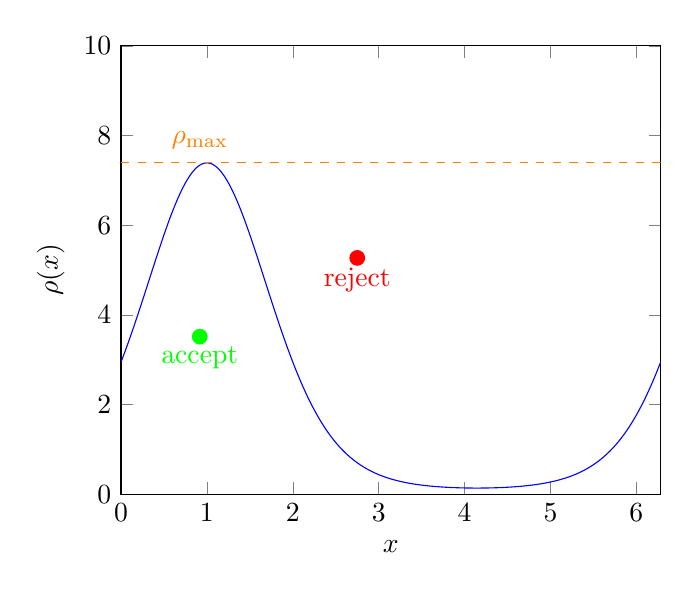
\begin{tikzpicture}

\begin{axis}[
    xlabel=$x$, ylabel=$\rho(x)$,
    xmin=0, xmax=2*pi,
    ymin=0, ymax=10
]
\addplot[blue, domain=0:2*pi, samples=1000] {exp(2*cos(deg(x-1))};
\addplot[orange, domain = 0:2*pi, dashed] {exp(2)};
\end{axis}
\fill[green] (1,2) circle (0.1) node[below] {accept};
\fill[red] (3,3) circle (0.1) node[below]{reject};
\node[orange] at (1,4.5) {$\rho_{\text{max}}$};
\end{tikzpicture} 


\end{document}